\chapter{LapOps Application}\label{manual}
This section describes, explains and shows the application that was created in this workshop. It contains a manual and additional informations for the correct usage of LapOps

\section{LapOps Manual}
The following section describes how the user can interact with LapOps and what he or she needs to do, to use it properly.

\subsection{Preparation}
Because we chose the near field sensor as a sensor to keep track of our laps, it is necessary to create a bride, or start/finish line, that is close enough to the device if the car travels through it. The distance between the bottom of the bride and the device has to be less than 3 centimetres. To confirm if the distance is small enough you can refer to our application. The pictures visible in figure \ref{LabOpsnearfield} show LabOps, when it needs to be put at the starting line. The GO button only appears when the near field sensor is active and therefore the laps can be started.

\begin{figure}[H]
	\centering
	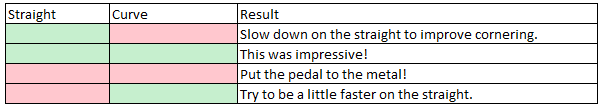
\includegraphics[scale= 0.9]{Pictures/StraightResultMapping.png}
	\caption{RC car with mounted device and bridge for a start/finish line}
	\label{startFinishLineWithRC}
\end{figure}

\begin{figure}[H]
	\begin{subfigure}[c]{0.4\textwidth}
		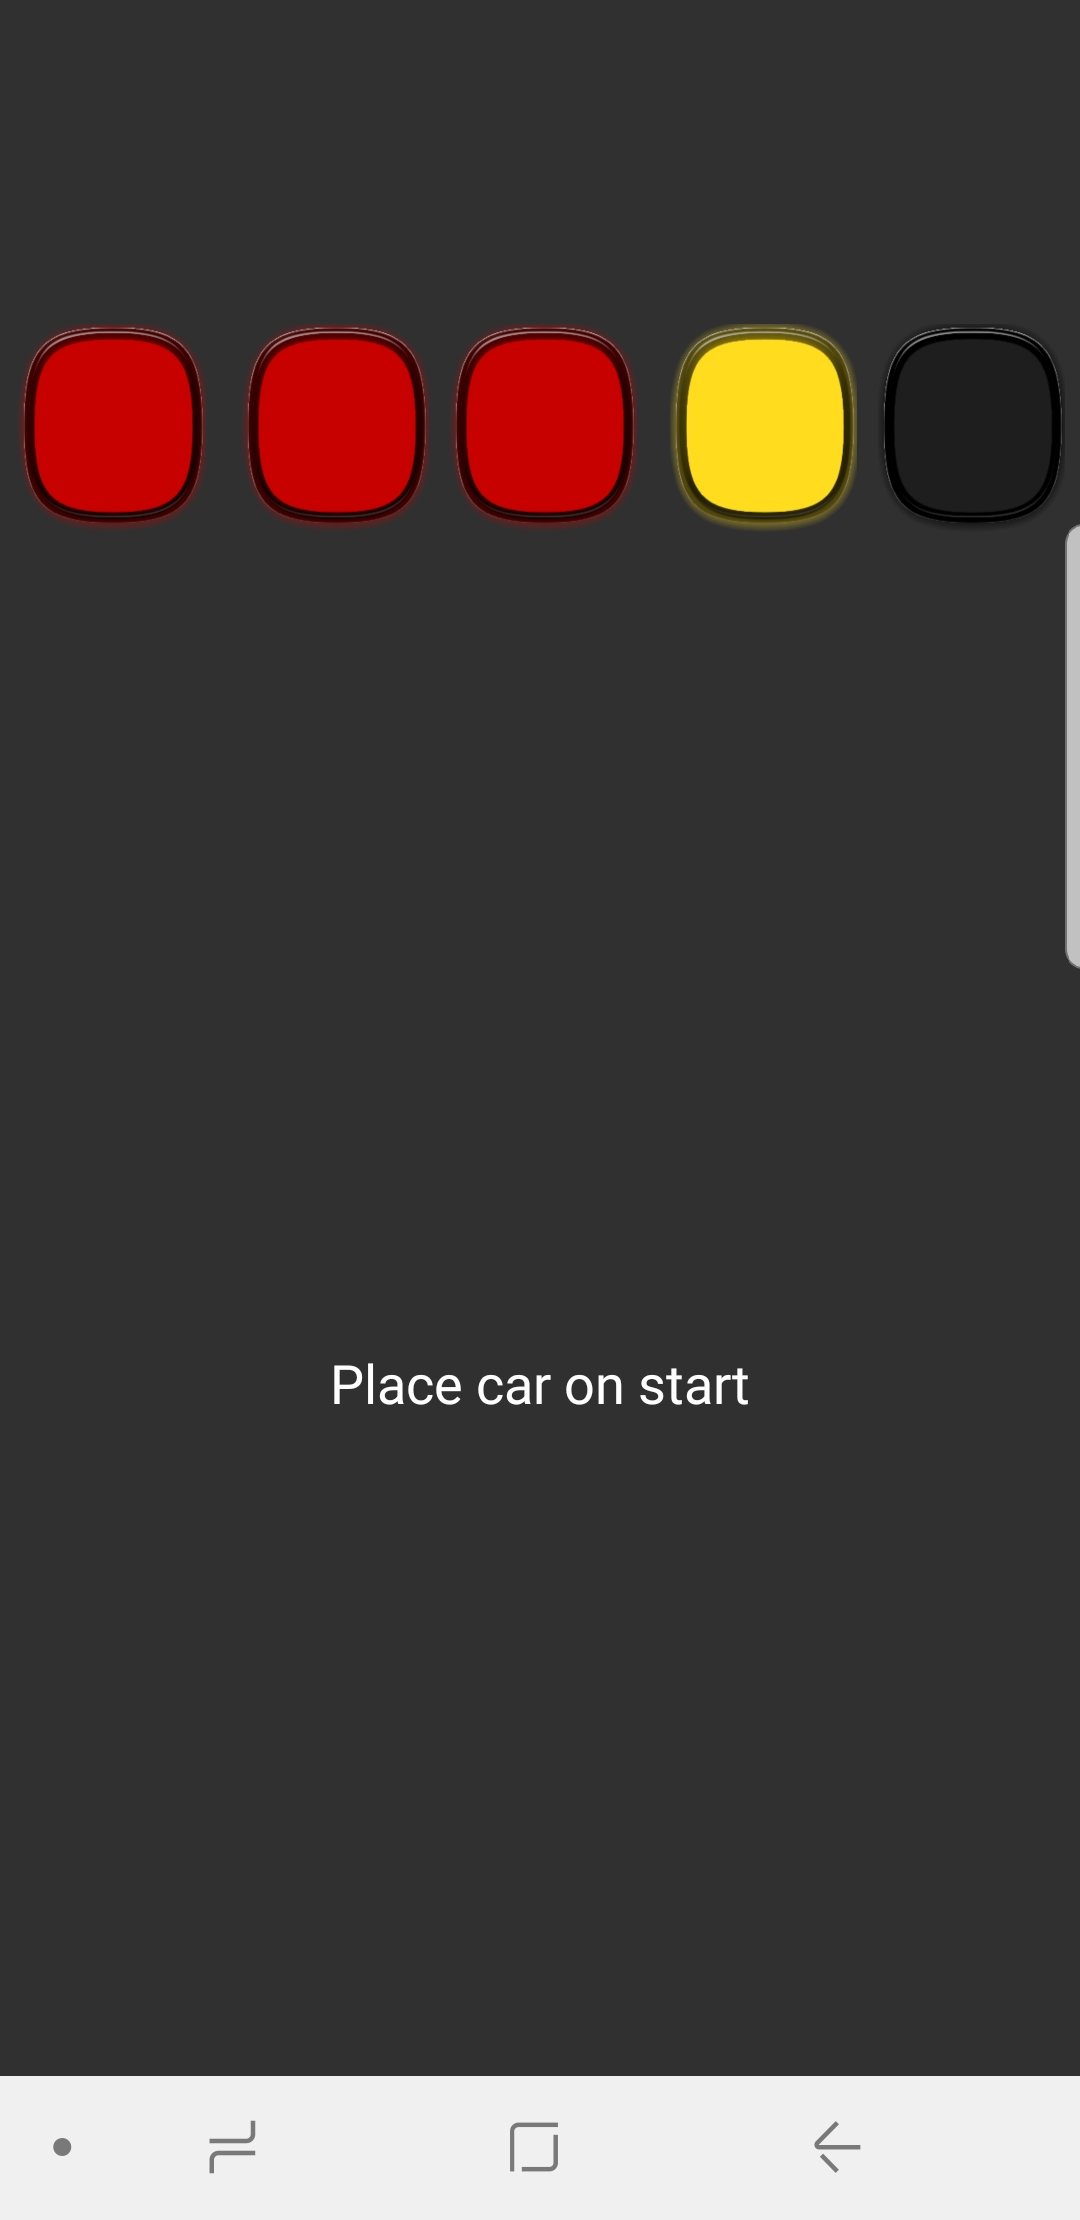
\includegraphics[width=\textwidth]{Pictures/App/PreNearFiled.jpg}
		\subcaption{Car needs to be put in position to activate near field sensor}
		
	\end{subfigure}
	\hfill
	\begin{subfigure}[c]{0.4\textwidth}
		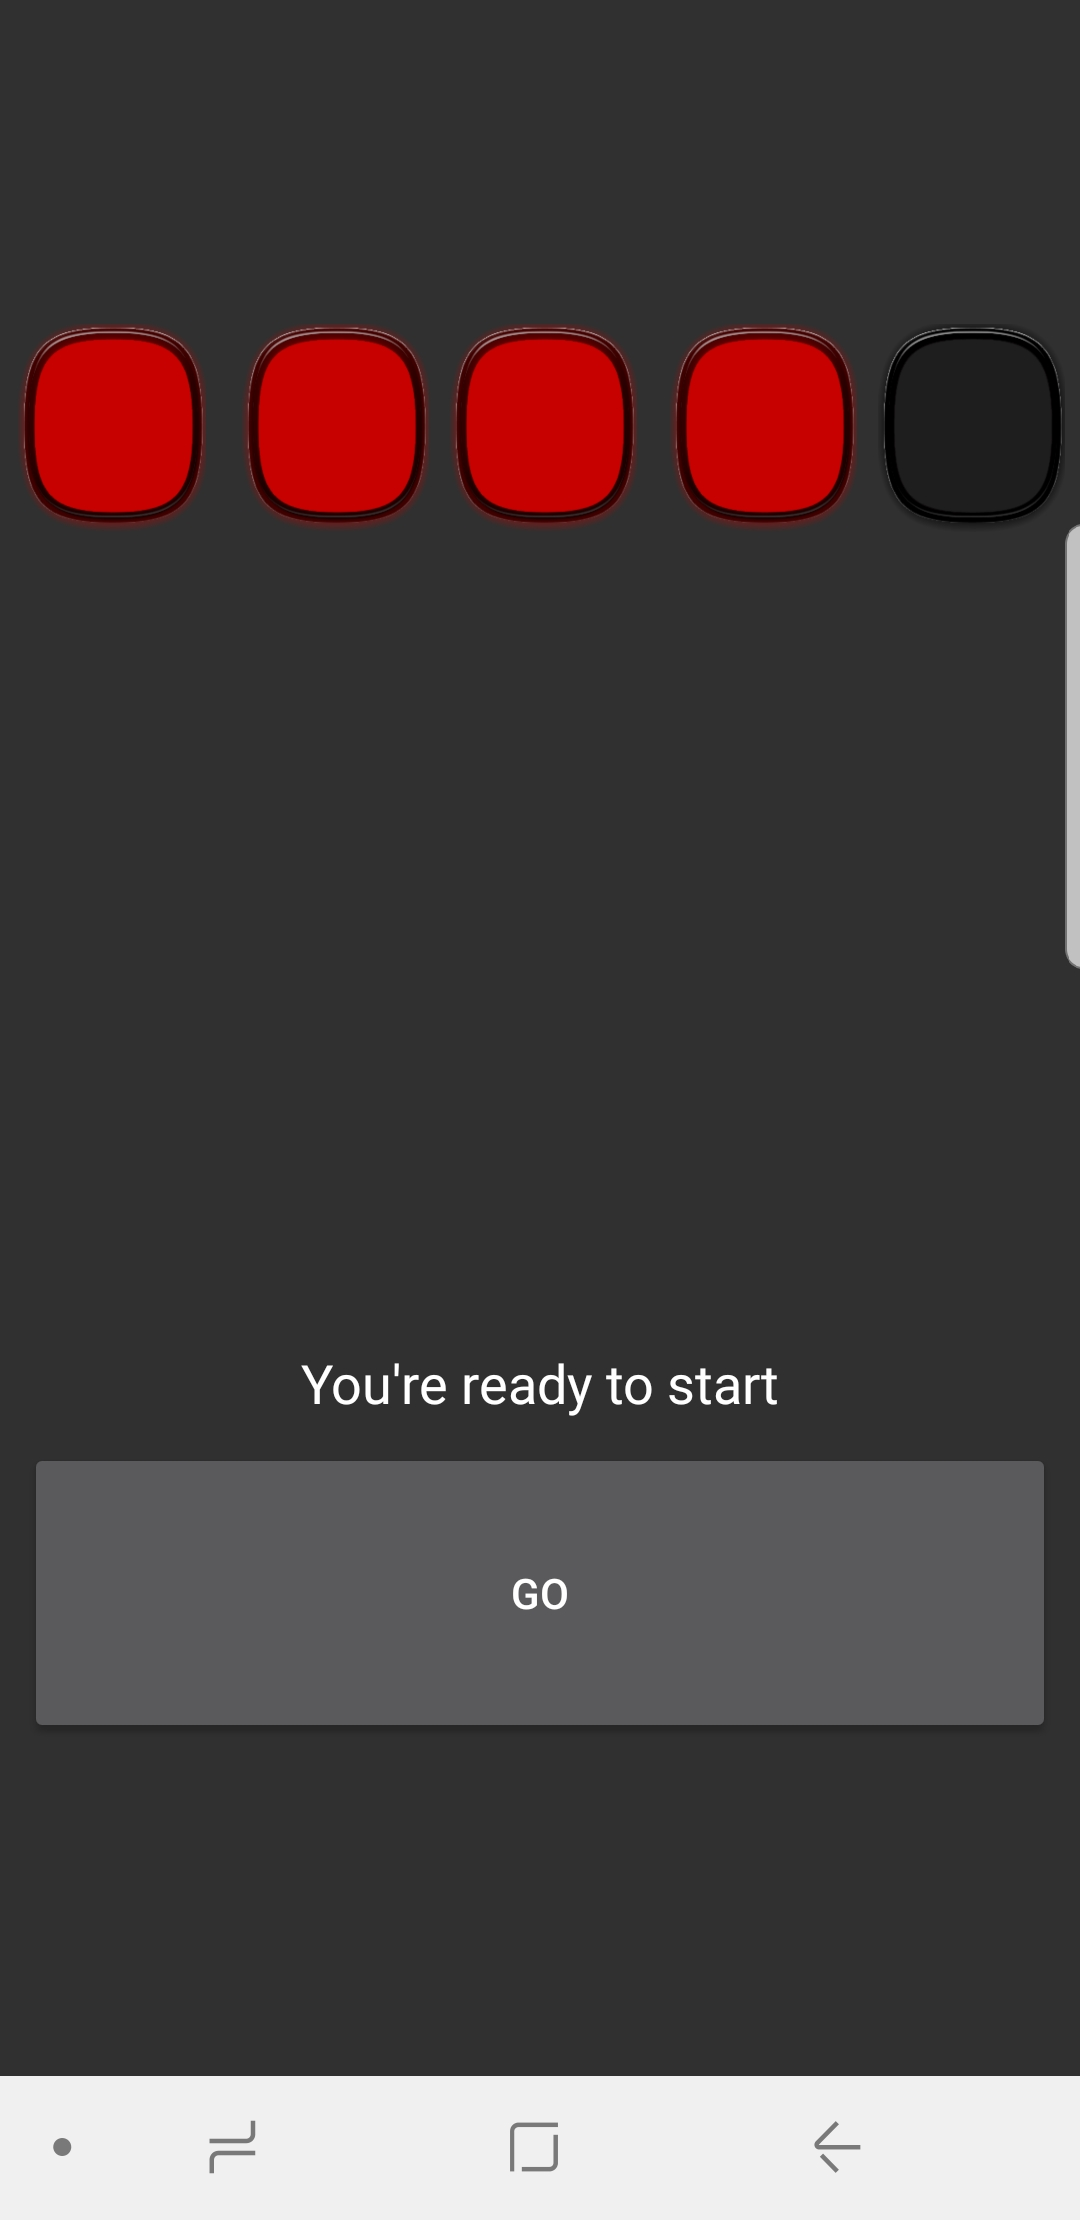
\includegraphics[width=\textwidth]{Pictures/App/FieldActivated.jpg}
		\subcaption{Near field sensor is activated and LapOps is ready to collect data}
		
	\end{subfigure}
	\caption{Overview of LapOps for starting phase}
	\label{LabOpsnearfield}
\end{figure}

\subsection{LapOps workflow for lap optimizations}
After doing the  it is pretty easy to use LapOps, the only thing that needs to be done is driving on a track. Please consider that it is important, that enough laps are driven for the system to recognize a pattern in the accelerometer data. In our tests 10 to 15 laps were mostly fine. After driving the laps, just stop the car and click on the finish button. After processing of the data, the result screen will be displayed. The first thing, that is visible will be the screen seen in figure \ref{LapOpsResult} (a). This overview lists all the driving laps and there state. Green represents the fastest driven lap in the current session. Yellow represents other laps, that are valid. These can be opened to view performance of the sections. The red laps are considered invalid. These happens if the track that the car drove was to different from the rest. After clicking on a valid lap(yellow) the screen visible in figure \ref{LapOpsResult} (b,c) will be visible. In this overview, the yellow represents an equal result to the fastest lap. The red color represents a way slower result and the green one is there to indicate a faster driven section, than the reference lap.
\begin{figure}[H]
	\begin{subfigure}[c]{0.32\textwidth}
		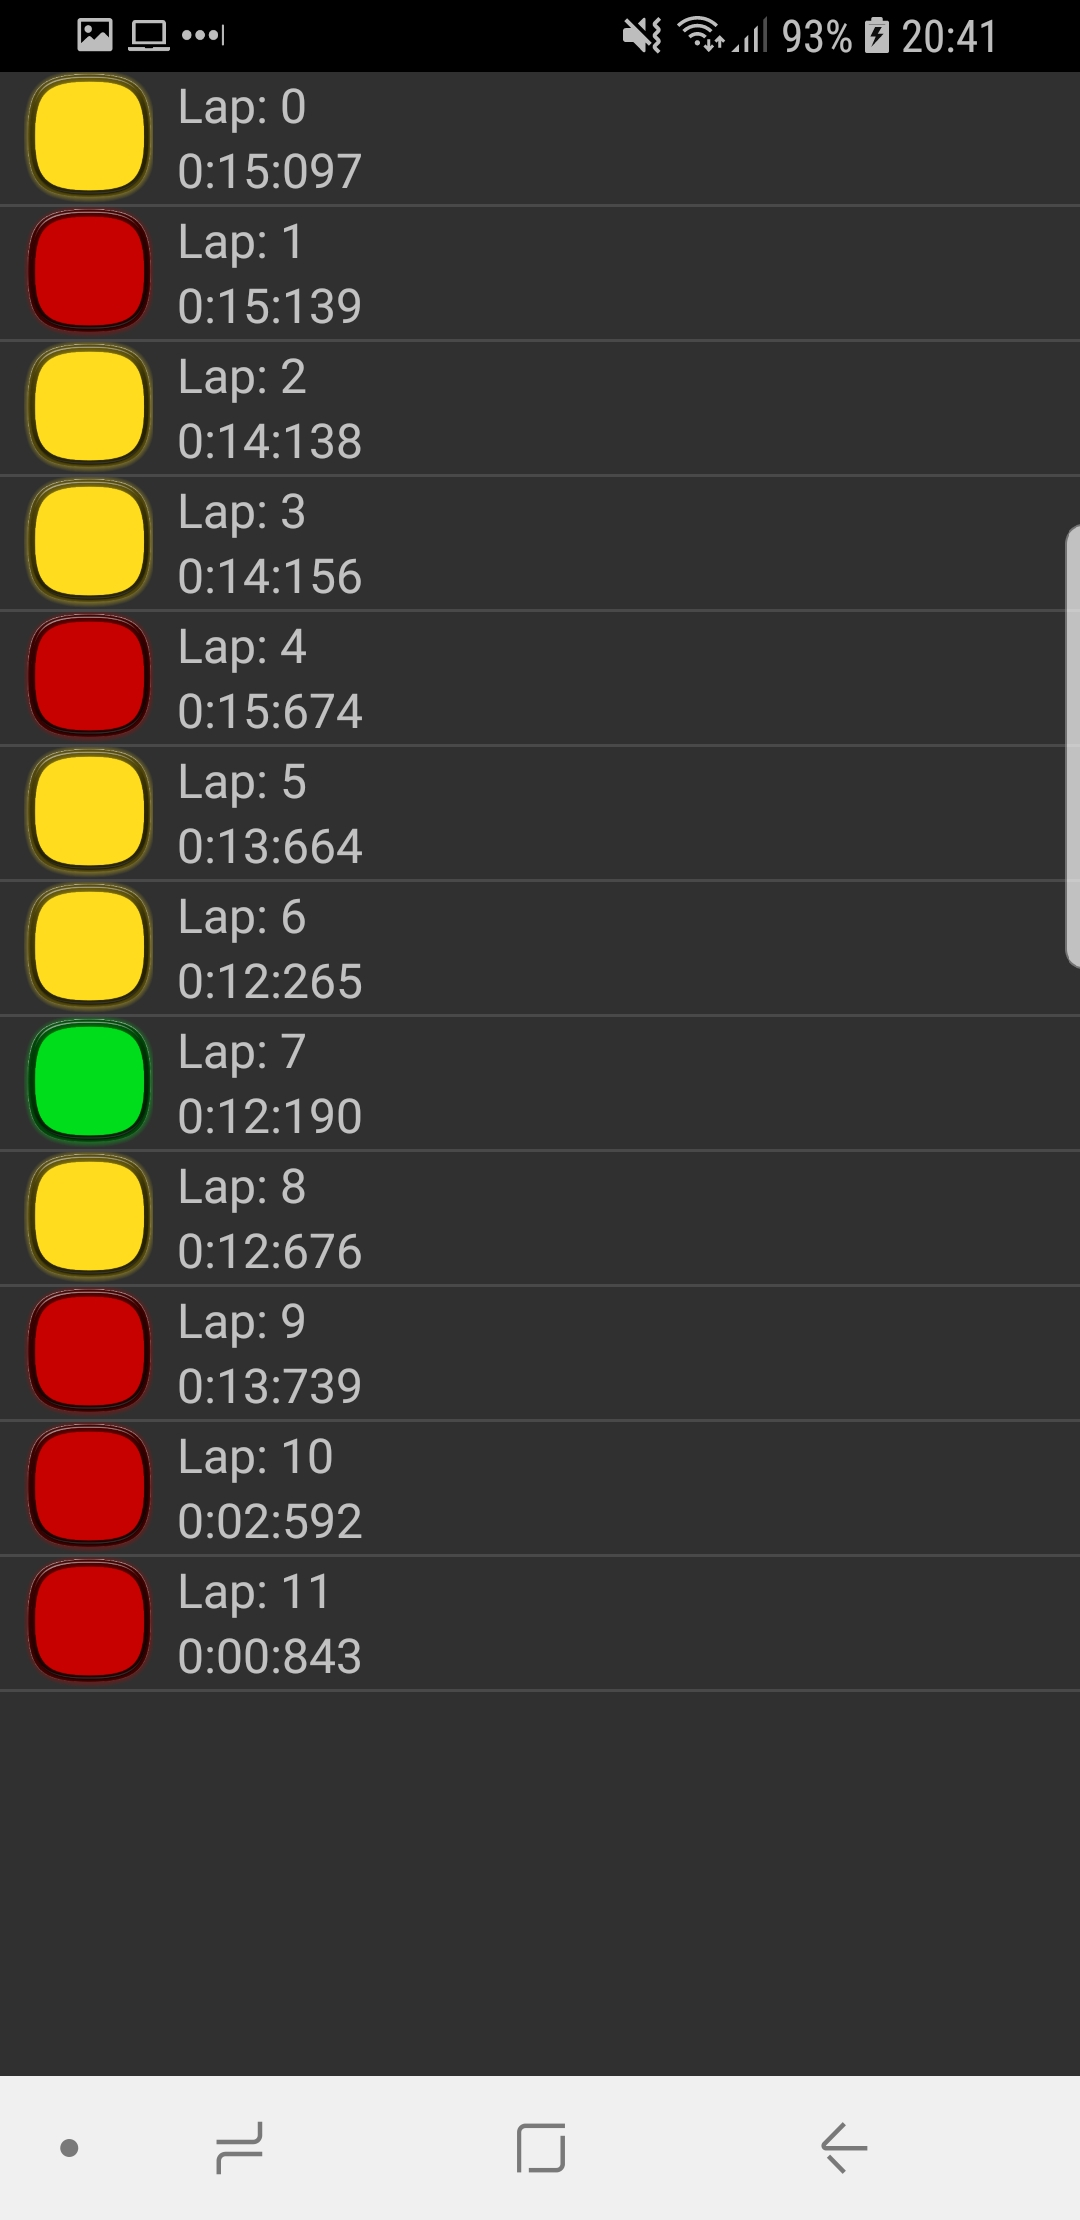
\includegraphics[width=\textwidth]{Pictures/App/LapList.jpg}
		\subcaption{Overview of the driven laps in a session}
		
	\end{subfigure}
	\hfill
	\begin{subfigure}[c]{0.32\textwidth}
		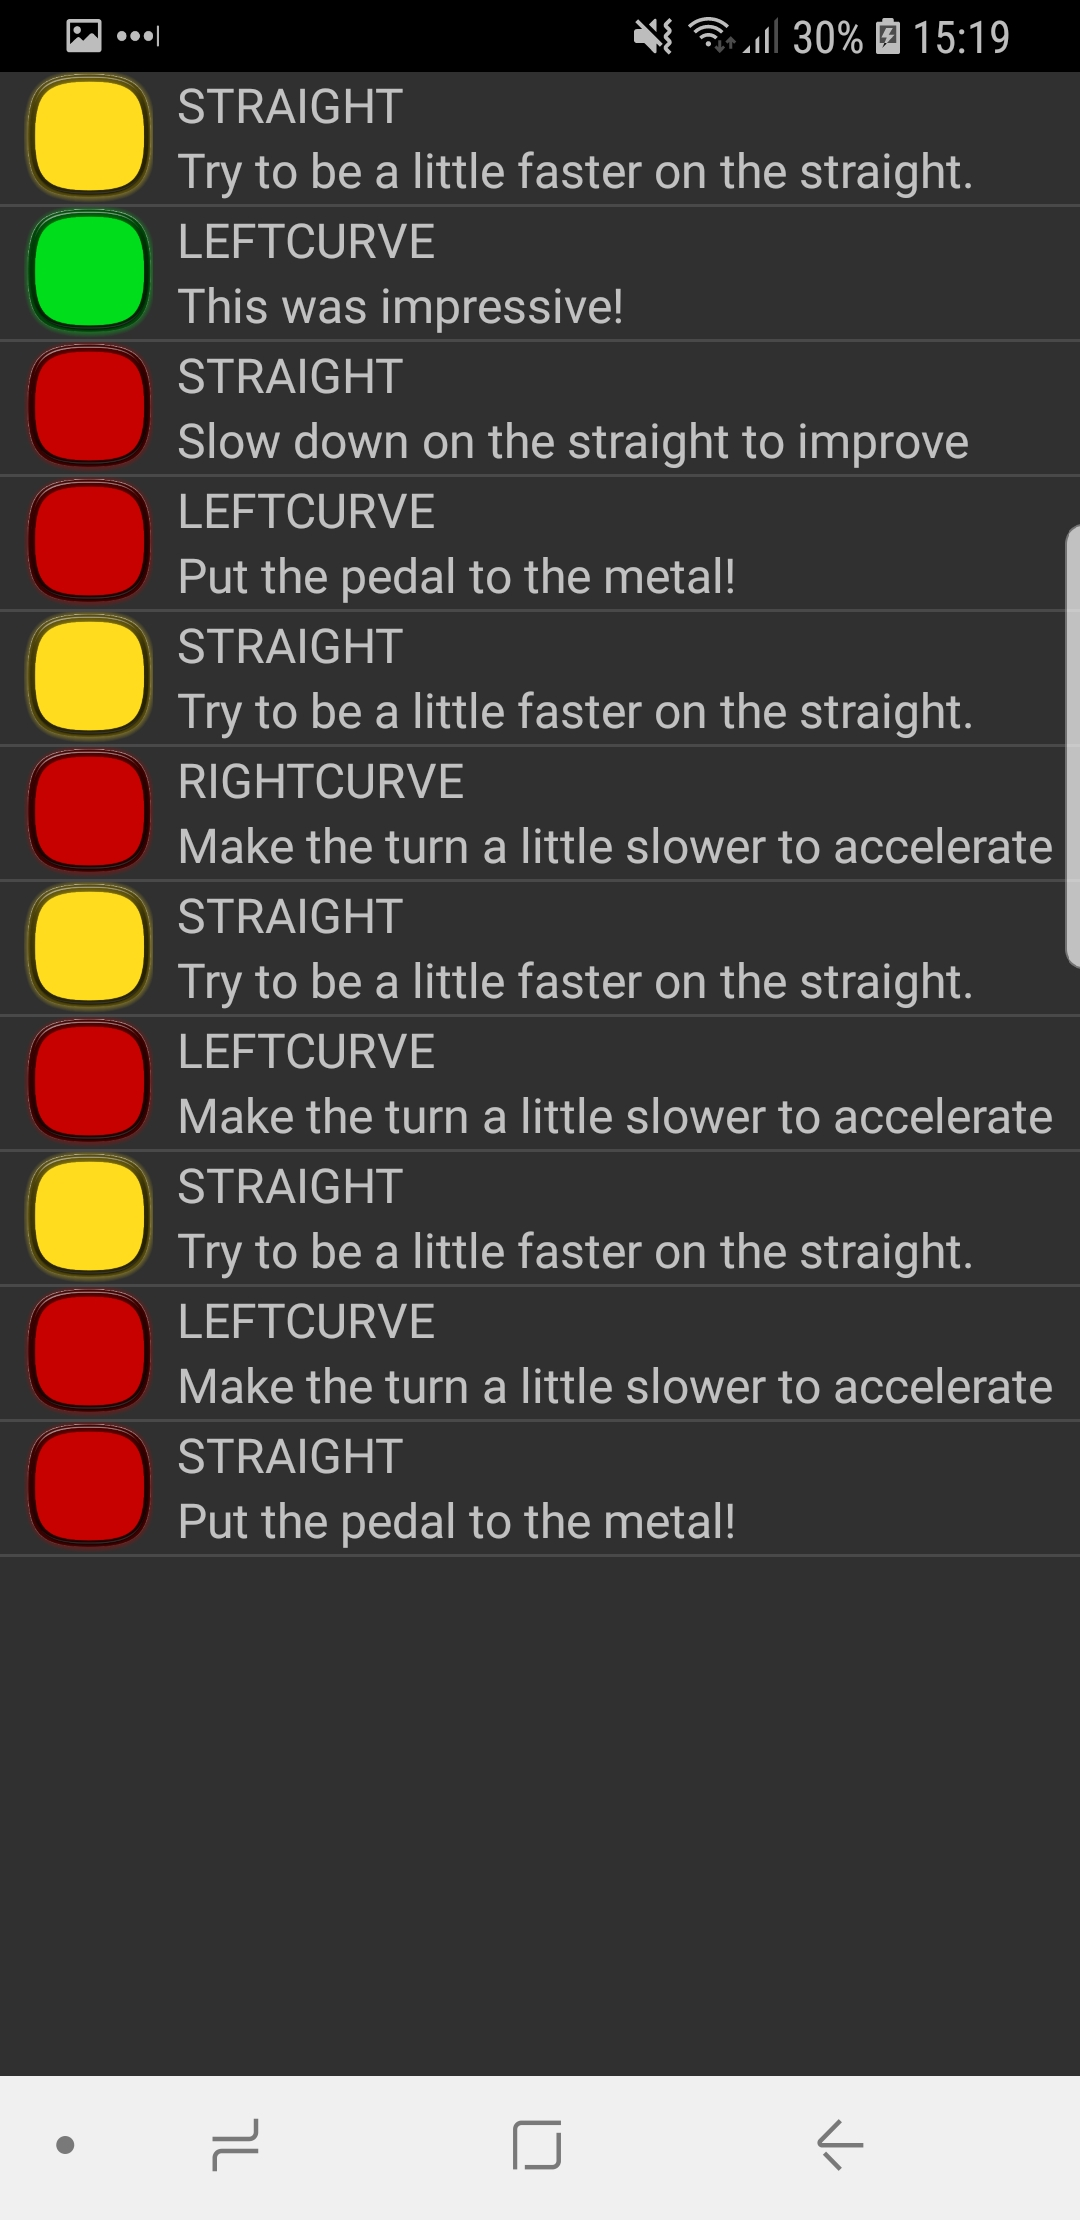
\includegraphics[width=\textwidth]{Pictures/App/SectionScreen1.jpg}
		\subcaption{First overview of the sections inside a lap}
		
	\end{subfigure}
	\hfill
	\begin{subfigure}[c]{0.32\textwidth}
		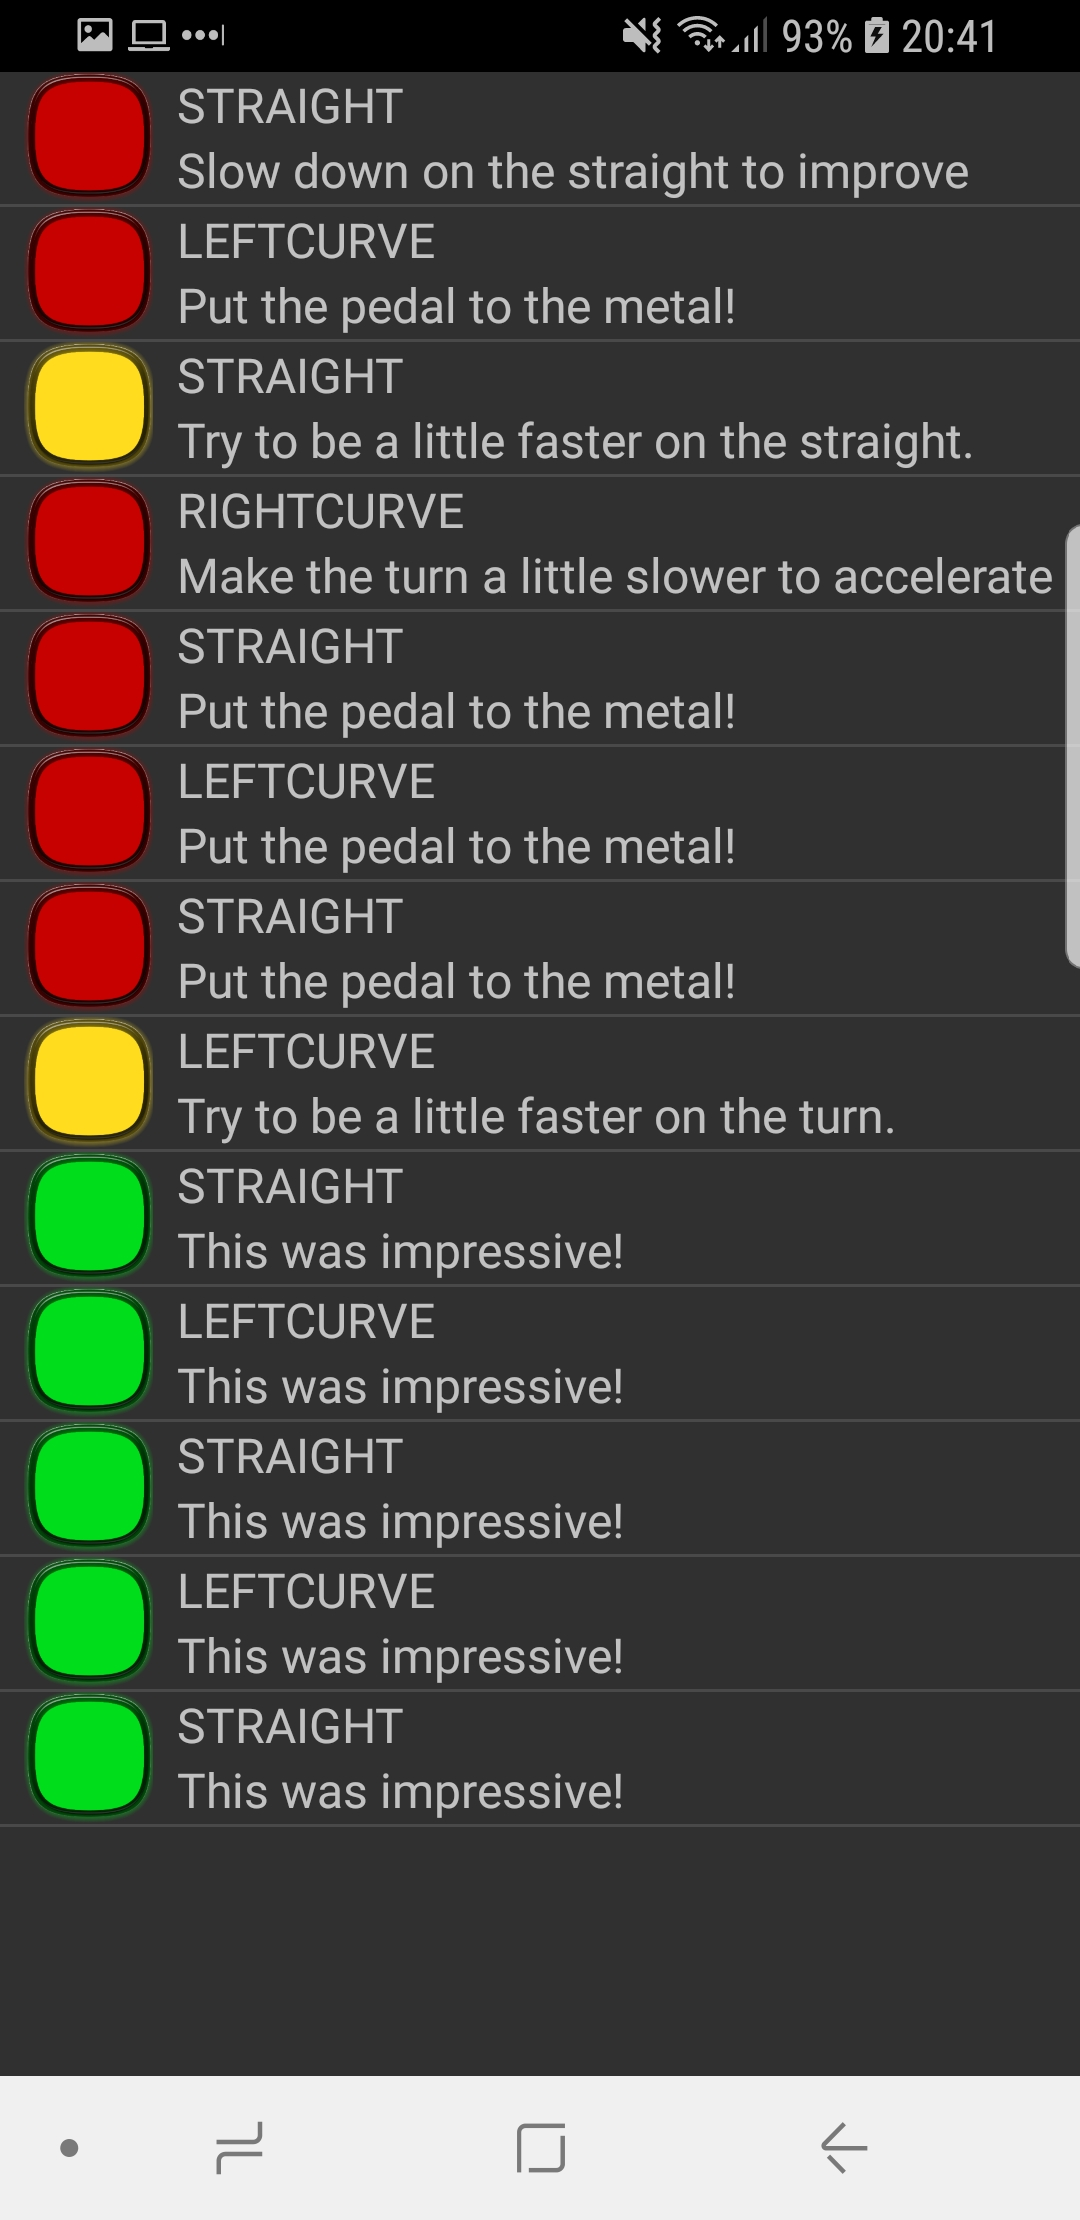
\includegraphics[width=\textwidth]{Pictures/App/SectionScreen2.jpg}
		\subcaption{Second overview of the sections inside a lap}
	\end{subfigure}

	\caption{Result screens of LapOps}
	\label{LapOpsResult}
\end{figure}
\newpage
\section{Additional information}
This section provides additional information of the project. 

\subsection{Issues with provided smartphone}
One big issue was the near field sensor of the provided Huawei smarthphone. The nearfield sensor is heavily delayed and does not register if driven to fast under the bridge. Therefore if there is a need to use the Huawei smarthphone please drive slowly under the bridge for the near field sensor to trigger. 

\subsection{Login for the different social channels}
The following section lists the login credentials for the social channels, that were used in this project.

\begin{tabular}{ l | p{5.6cm} | l }
	Website & Login & Link \\ \hline
	youtube.com & Login: dsce.team.d@gmail.com Pw: Secret & 6 \\
	hackster.io & Login: dsce.team.d@gmail.com Pw: Secret & 6 \\
\end{tabular}
